%% these.tex
%% Copyright 2010 Luca De Feo
%% All rights reserved


\section{Experimental results}
\label{sec:artin-benchmarks}

We discuss here the implementation of the algorithms of this Chapter
and some experimental results.

\paragraph{Implementation}
We packaged the algorithms of this chapter in a \texttt{C++} library
called \texttt{FAAST} and made it available under the terms of the
\texttt{GNU GPL} software license from
\url{http://www.lix.polytechnique.fr/Labo/Luca.De-Feo/FAAST/}.

\texttt{FAAST} is implemented on top of the \texttt{NTL}
library~\cite{shoup2003ntl} which provides the basic univariate
polynomial arithmetic needed here. Our library handles three NTL
classes of finite fields: \texttt{GF2} for $p=2$, \texttt{zz\_p} for
word-size $p$ and \texttt{ZZ\_p} for arbitrary $p$; this choice is made
by the user at compile-time through the use of \texttt{C++} templates
and the resulting code is thus quite efficient.  Optionally,
\texttt{NTL} can be combined with the \texttt{gf2x}
package~\cite{gf2x} for better performance in the $p=2$ case, as we
did in our experiments.

All the algorithms of
Sections~\ref{sec:fast-tower}--\ref{sec:pseudotrace-frobenius} are
faithfully implemented in \texttt{FAAST}. The algorithms
\titleref{alg:applyisomorphism} and \titleref{alg:applyinverse} have
slightly different implementations \texttt{toUnivariate()} and
\texttt{toBivariate()} that allow more flexibility. Instead of being
recursive algorithms doing the change to and from the multivariate
basis $\basis{B}'_i=\{{x_0'}^{e_0}\cdots {x_i'}^{e_i}\}$, they only
implement the change to and from the bivariate basis
\begin{equation}
  \label{eq:278}
  \basis{D}'_i=\{{x_{i-1}}^{e_{i-1}}{x_i'}^{e_i} \;|\;0\le
  e_{i-1}<p^{i-1}d,\; 0\le e_i<p\}
  \text{.}
\end{equation}
Equivalently, this amounts to
switch between the representations
\begin{equation}
  \wrt\U_i \quad\text{and}\quad
  \wrt\U_{i-1}[X_i']/({X_i'}^p-X_i'-\gamma_{i-1}')
  \text{.}
\end{equation}
The same result as one call to \titleref{alg:applyisomorphism} or
\titleref{alg:applyinverse} can be obtained by $i$ calls to
\texttt{toUnivariate()} and \texttt{toBivariate()} respectively.

\pdfmctwo{I tried to be more clear on this. I do not know if I
  succeeded.}  However, more freedom is allowed in the case where
several generic Artin-Schreier towers, say $(\U_0',\ldots,\U_k')$ and
$(\U_0'',\ldots,\U_k'')$, are built using the algorithms of Section
\ref{sec:couveignes-algorithm}. In fact it is possible, for example,
to see $\U_k''$ as an extension field of $\U'_k$ by first converting
to the basis $\basis{D}''_k$ and then recursively to
$\basis{D}'_{k-1},\ldots,\basis{D}'_1$. More generally, this allows
the user to build a new Artin-Schreier tower
$(\U_0''',\ldots,\U_k''')$ by taking at each level either
$\U_i'''=\U_i'$ or $\U_i'''=\U_i''$.  In other words this allows the
user to \emph{zig-zag} in the lattice of finite fields as in
Figure~\ref{fig:lattice}.

\begin{figure}
  \centering
  \begin{equation*}
    \xymatrix@C=1cm{
      & v\wrt\U_k \ar@{<--}@(r,u)[dr] \\
      \U_k'\ar@{-}[r]^{\sigma'} & \U_k\ar@{-}[d] & \U_k''\ar@{-}[l]_{\sigma''} \ar@{--}@(d,u)[dll]\\
      \U_{k-1}'\ar@{-}[r]^{\sigma'} \ar@{--}@(d,u)[drr] & \U_{k-1}\ar@{.}[d] & \U_{k-1}''\ar@{-}[l]_{\sigma''}\\
      \U_1'\ar@{-}[r]^{\sigma'} & \U_1\ar@{-}[d] & \U_1''\ar@{-}[l]_{\sigma''}\ar@{-->}[d]\\
      & \U_0 & *[r]{v\wrt\U_0[x_1'',\ldots,x_{k-1}',x_k'']}
    }
  \end{equation*}
  \caption{An example of conversion from the univariate basis to the
    multivariate basis of the tower $(\U_0,\U_1'',\ldots,\U_{k-1}',\U_k'')$.}
  \label{fig:lattice}
\end{figure}

Besides the algorithms of this Chapter, \texttt{FAAST} also implements
the algorithms described in Section~\ref{sec:C2-AS-FI} for minimal
polynomials, evaluation and interpolation.

\pdfmcthree{Moved to Magma 2.16}
\paragraph{Experimental results} We compare our timings with those
obtained in Mag\-ma 2.16~\cite{MAGMA} for similar questions.  All
results are obtained on an Intel Xeon E5520 (2.26GHz). Our experiments
revealed a regression in the performances of Magma 2.16, concerning
one algorithm. When such difference is noticeable, we also plot the
timings obtained with Magma 2.11 on an equivalent machine (Intel Xeon
E5430).


The experiments for the \texttt{FAAST} library were only made for the
classes \texttt{GF2} and \texttt{zz\_p}. The class \texttt{ZZ\_p} was
left out because all the primes that can be reasonably handled by our
library fit in one machine-word. In Magma, there exist several ways to
build field extensions:
\begin{itemize}
\item \texttt{quo<U|P>} builds the quotient of the univariate
  polynomial ring $U$ by $P \in U$ (written magma(1) hereafter);
\item \texttt{ext<k|P>} builds the extension of the field $k$ by $P
  \in k[X]$ (written magma(2));
\item \texttt{ext<k|p>} builds an extension of degree $p$ of $k$
  (written magma(3)).
\end{itemize}
We made experiments for each of these choices where this makes sense.

The parameters to our algorithms are $(p,d,k)$. Thus, our experiments
describe the following situations:

\begin{itemize}
\item \emph{Increasing the height $k$.} Here we take $p=2$ and $d=1$
  (that is, $\U_0=\F_2$); the $x$-coordinate gives the number of
  levels we construct and the $y$-coordinate gives timings in seconds,
  in \emph{logarithmic} scale.

  This is done in Figure~\ref{fig:height}. We let the height of the
  tower increase and we give timings for (1) building the tower of
  Section~\ref{sec:fast-tower} and (2) computing an isomorphism with a
  random arbitrary tower as in Section~\ref{sec:couveignes-algorithm}.
  In the latter experiment, only the magma(2) approach was meaningful
  for Magma.
\item \emph{Increasing the degree $d$ of $\U_0$.} Here we take $p=5$
  and we construct $2$ levels; the $x$-coordinate gives the degree $d
  = [\U_0:\F_p]$ and the $y$-coordinate gives timings in seconds.
  This is done in Figure~\ref{fig:p-d} (left).
\item \emph{Increasing $p$.} Here we take $d=1$ (thus $\U_0=\F_p$) and
  we construct $2$ levels; the $x$-coordinate gives the characteristic
  $p$ and the $y$-coordinate gives timings in seconds.  This is done
  in Figure~\ref{fig:p-d} (right).
\end{itemize}



\begin{figure}
  \centering
  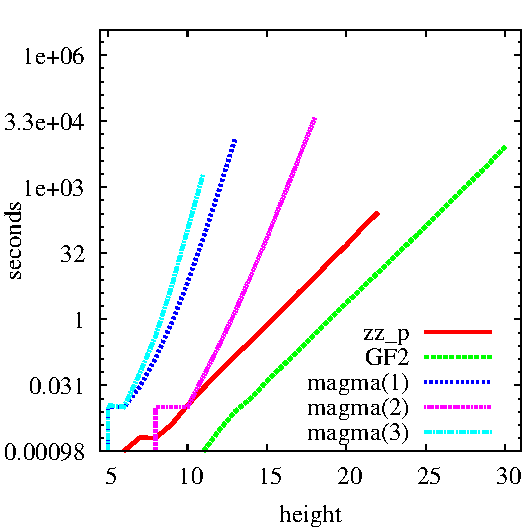
\includegraphics[height=0.5\textwidth]{artin/build1}
  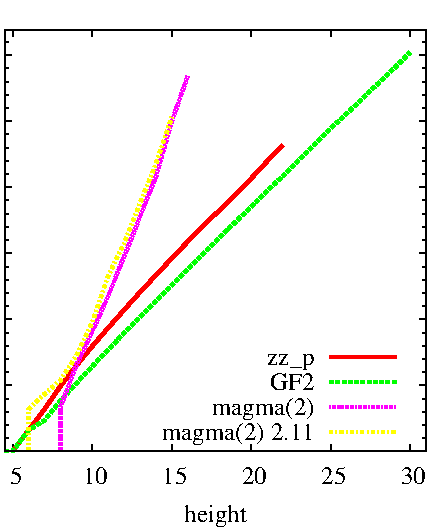
\includegraphics[height=0.5\textwidth]{artin/iso1}
  
  \caption{Build time (left) and isomorphism time (right) with respect to tower height. Plot is in logarithmic scale.}
  \label{fig:height}
\end{figure}

\begin{figure}
  \centering
  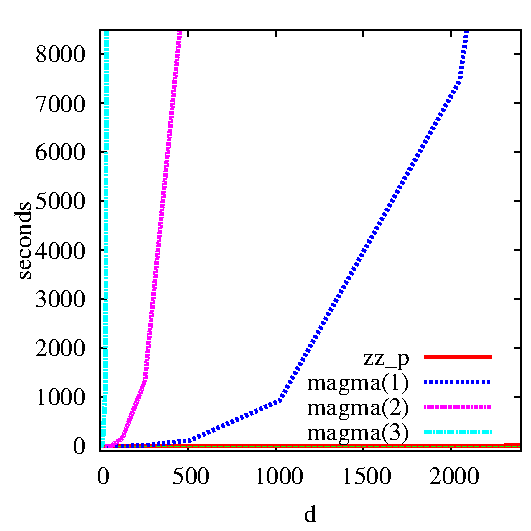
\includegraphics[height=0.5\textwidth]{artin/build-d}
  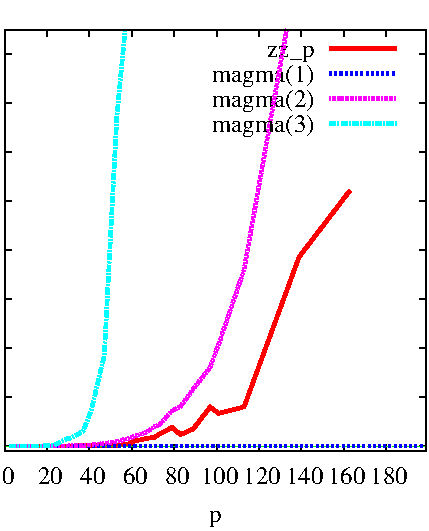
\includegraphics[height=0.5\textwidth]{artin/build-p}
  
  \caption{Build times with respect to $d$ (left) and $p$ (right).}
  \label{fig:p-d}
\end{figure}

\pdfmcthree{A little comment on magma(2) for p increasing.}
The timings of our code are significantly better for increasing height
or increasing $d$. Not surprisingly, for increasing $p$, the magma(1)
approach performs better than any other: the \texttt{quo} operation
simply creates a residue class ring, regardless of the
(ir)reducibility of the modulus, so the timing for building two levels
barely depend on $p$. The most adapted approach for this situation
presumably is magma(2); yet we notice that \texttt{FAAST} has
reasonable performances for characteristics up to about $p=50$.

In Tables~\ref{tab:arith-gf2} and~\ref{tab:arith-zzp} we provide some
comparative timings for the different arithmetic operations provided
by \texttt{FAAST}. The column ``Primitive'' gives the time taken to
build one level of the primitive tower (this includes the
precomputation of the data as described in
Subsection~\ref{sec:level-embedding:lift-up}); the other entries are
self-explanatory. Product and inversion are just wrappers around
\texttt{NTL} routines: in these operations we did not observe any
overhead compared to the native \texttt{NTL} code. 

\begin{table}
  \centering
  \begin{tabular}{l r r r r r r r}
    \hline
    \small level & \small Primitive & \small Push-d. & \small Lift-up & \small Product & \small Reciprocal & \small apply $\sigma^{-1}$ & \small apply $\sigma$ \\
    \hline
    19 &  1.143 & 0.304 &  1.265 & 0.039 &  0.649 &  0.652 &  1.290\\
    20 &  2.566 & 0.609 &  2.796 & 0.081 &  1.544 &  1.314 &  2.602\\
    21 &  5.686 & 1.225 &  6.147 & 0.187 &  3.598 &  2.409 &  2.668\\
    22 & 12.660 & 2.515 & 13.746 & 0.463 &  8.355 &  5.565 & 11.179\\
    23 & 28.511 & 5.295 & 31.200 & 1.046 & 19.522 & 12.323 & 24.740
  \end{tabular}
  \caption{Some timings in seconds for arithmetics in a generic tower built over $\F_2$ using \texttt{GF2}.}
  \label{tab:arith-gf2}
\end{table}

\begin{table}
  \centering
  \begin{tabular}{l r r r r r r r}
    \hline
    \small level & \small Primitive & \small Push-d. & \small Lift-up & \small Product & \small Reciprocal & \small apply $\sigma^{-1}$ & \small apply $\sigma$ \\
    \hline
    18 &  13.618 &  0.884 &  13.712 & 0.476 &  10.753 &  1.337 &  3.578\\
    19 &  30.288 &  1.814 &  30.432 & 1.001 &  23.046 &  2.850 &  7.798\\
    20 &  65.632 &  3.953 &  66.889 & 2.106 &  51.544 &  6.564 & 18.141\\
    21 & 128.190 &  8.347 & 131.271 & 4.791 & 121.349 & 14.396 & 39.296\\
    22 & 296.671 & 11.396 & 298.541 & 6.413 & 249.520 & 28.851 & 86.628
  \end{tabular}
  \caption{Some timings in seconds for arithmetics in a generic tower built over $\F_2$ using \texttt{zz\_p}.}
  \label{tab:arith-zzp}
\end{table}


Finally, we mention the cost of precomputation. The precomputation of
the images of $\sigma$ as explained in
Section~\ref{sec:couveignes-algorithm} is quite expensive; most of it
is spent computing pseudotraces. Indeed it took one week to precompute
the data in Figure~\ref{fig:height} (right), while all the other data
can be computed in a few hours. There is still space for some minor
improvement in \texttt{FAAST}, mainly tweaking recursion thresholds
and implementing better algorithms for small and moderate input
sizes. Yet we think that only a major algorithmic improvement could
consistently speed up this phase.



% Local Variables: 
% mode:flyspell
% ispell-local-dictionary:"american"
% TeX-master: "../these"
% mode: TeX-PDF
% mode: reftex
% End: 
%
% LocalWords:  univariate isogeny Couveignes isogenies Artin Schreier
